\documentclass[11pt]{article}
\usepackage{geometry}                % See geometry.pdf to learn the layout options. There are lots.
\geometry{letterpaper}                   % ... or a4paper or a5paper or ... 
%\geometry{landscape}                % Activate for for rotated page geometry
%\usepackage[parfill]{parskip}    % Activate to begin paragraphs with an empty line rather than an indent
\usepackage{graphicx}
\usepackage{amssymb}
\usepackage{epstopdf}
\DeclareGraphicsRule{.tif}{png}{.png}{`convert #1 `dirname #1`/`basename #1 .tif`.png}

%

\usepackage[nottoc]{tocbibind} %for table of contents
\usepackage{amsmath}
\usepackage{wrapfig}

\title{Computational Physics Project A \\ Modelling Single \& Double Pendulum Systems Computationally}
\author{Joshua Maxey}
%\date{}                                           % Activate to display a given date or no date

\begin{document}
\maketitle

\begin{center}
The Euler, Leapfrog and Runge-Kutta (4th order) numerical methods are used to computationally model a single pendulum system. By varying system and method parameters limits are found for the stabiity of these methods ad their suitability for oscillatory problems. The conclusions of this preliminary investigation feed into the more complex double pendulum system. THIS ISN'T OVER!
\end{center}

\tableofcontents
\pagebreak

\section{Introduction}
Computational models of physical systems require us to discretise continuous variables (often, but not exclusively, time). Numerical methods approximate derivatives to provide a means to solving differential equaitons computationally. The three numerical methods investigated in this project are Euler's method, the Leapfrog method and the 4th order Runge-Kutta method.

\section{The Single Pendulum}
\subsection{Theory}
\subsubsection*{System Description \& Parameters}
The idealised single pendulum system comprises a fixed mass $m$ attached to the end of a massless rod of length $l$ suspended from a pivot which applies a friction that is characterised by the damping constant $\gamma$. It is depicted in figure \ref{fig:sp_diag}.

%\setlength{\columnsep}{30pt} %adjusts horizontal padding
\begin{wrapfigure}{r}{0pt}
\vspace{-20pt}
\hspace{5pt}
\includegraphics[height=0.3\textheight]{img/sp_diag.png}
\caption{The single pendulum notation used throughout this report.}
\label{fig:sp_diag}
%\vspace{-30pt}
\end{wrapfigure}

\subsubsection*{Equations of Motion}
The motion of the pendulum is defined by equation \ref{eq:eom_sp} where $\theta$ is the angle the pendulum makes with the vertical.
\begin{equation} \label{eq:eom_sp}
ml\frac{d^2 \theta}{dt^2} = -mg\sin(\theta) - \gamma\frac{d\theta}{dt}
\end{equation}
By applying the small angle approximation, choosing dimensionless units of time to yeild reduced time, $\widetilde{t}$, such that
\begin{equation} \label{eq:const_def}
\widetilde{t} = t\sqrt{\frac{l}{g}} \;\;\; \text{and choosing} \;\;\; \beta = \frac{\gamma}{m \sqrt{gl}}
\end{equation}
equation \ref{eq:eom_sp} reduces to
\begin{equation} \label{eq:eomsp_reduced}
\frac{d^2 \theta}{d\widetilde{t}^2} = \theta - \beta\frac{d\theta}{d\widetilde{t}}
\end{equation}

This can be expressed as a pair of coupled first order differential equations where $\omega$ is the rate of change of $\theta$ with respect to reduced time. They are presented in equation \ref{eq:coupled_1_order}.
\begin{equation} \label{eq:coupled_1_order}
\frac{d}{d\widetilde{t}} \begin{pmatrix}\theta \\ \omega \end{pmatrix} = \begin{pmatrix} 0 & 1 \\ -1 & -\beta \end{pmatrix} \begin{pmatrix}\theta \\ \omega \end{pmatrix}
\end{equation}
\subsubsection*{A Computer Model for the Single Pendulum System}
\subsubsection*{Euler's Method}
Euler's method is the simplest numerical method employed. It is obtained by Taylor expanding our function at an advanced time step $t$ + $h$ and truncating the result after the first two terms. As such, it is accurate to $O(h^2)$. 

Defining \underline{$L$} as the 2x2 matrix from \ref{eq:coupled_1_order} we can create the update matrix \underline{$T$} where $\underline{T}$ is defined as $\underline{I}$ + $h$ $\underline{L}$. To apply Euler's method we simply multiply the position vector at the current time step by this update matrix to find the values of $\theta$ and $\omega$ at the next time step. Hence,
\begin{equation} \label{eq:euler_seperate}
\begin{split}
\theta_{n+1} &= \theta_{n} + h\omega_{n} \\
\omega_{n+1} &= -h\theta_{n} + (1 -h \beta)\omega_{n}
\end{split}
\end{equation}

\subsubsection*{The Leapfrog Method}
The Leapfrog method is the simplest finite difference method that requires the storing of system variables at a previous timestep. It produces a gradient estimate from $y_{n-1}$ and $y_{n}$ which it uses to calculate $y_{n+1}$.  Using our notation, the Leapfrog method can be expressed as
\begin{equation} \label{eq:lf_vector}
\begin{pmatrix}\theta_{n+1} \\ \omega_{n+1} \end{pmatrix} = \begin{pmatrix}\theta_{n-1} \\ \omega_{n-1} \end{pmatrix} + 2 h \underline{L} \cdot \begin{pmatrix}\theta_{n} \\ \omega_{n} \end{pmatrix}
\end{equation}
These are manifest in code as equations \ref{eq:lf_seperate}
\begin{equation} \label{eq:lf_seperate}
\begin{split}
\theta_{n+1} &= \theta_{n-1} + 2h\omega_{n} \\
\omega_{n+1} &= \omega_{n-1} - 2h( \theta_{n} + \beta \omega )
\end{split}
\end{equation}

\subsubsection*{4th Order Runge-Kutta Method}
The Runge-Kutta method provide a generalisation for taking any number of gradients and producing a weighted average of them to predict the next value of $y$. This investigation employs the 4th order Runge-Kutta method (RK4). It is the highest order (and therefore most accurate) Runge-Kutta method where the number of evaulations required per step is less than or equal to the order of error. It is fourth order accurate; $O(h^4)$.

Although it requires significantly more evaluations per time step, the RK4 method is more computationally efficient due to its ability to remain accurate for much larger values of $h$. The set of equations \ref{eq:rk4_vector} show the four evaluations required before one can calculate the variables at the next time step.

\begin{equation} \label{eq:rk4_vector}
\begin{split}
\underline{k}_{1} &= h \underline{L} \cdot \underline{y}_{n}  \\
\underline{k}_{2} &= h \underline{L} \cdot ( \underline{y}_{n} + \frac{1}{2} \underline{k}_{1}) \\
\underline{k}_{3} &= h \underline{L} \cdot ( \underline{y}_{n} + \frac{1}{2} \underline{k}_{2}) \\
\underline{k}_{4} &= h \underline{L} \cdot ( \underline{y}_{n} + \underline{k}_{3}) \\
\underline{y}_{n+1} &= \underline{y}_{n} + \frac{1}{6} ( \underline{k}_{1} + 2\underline{k}_{2} + 2\underline{k}_{3} + \underline{k}_{4}) \\
\text{where} \;\;\;\; \underline{y}_{n} &= \begin{pmatrix}\theta_{n} \\ \omega_{n} \end{pmatrix}
\end{split}
\end{equation}

\subsection{Method}
\subsection{Results \& Discussion}

\setlength{\columnsep}{30pt} %adjusts horizontal padding
\begin{figure}
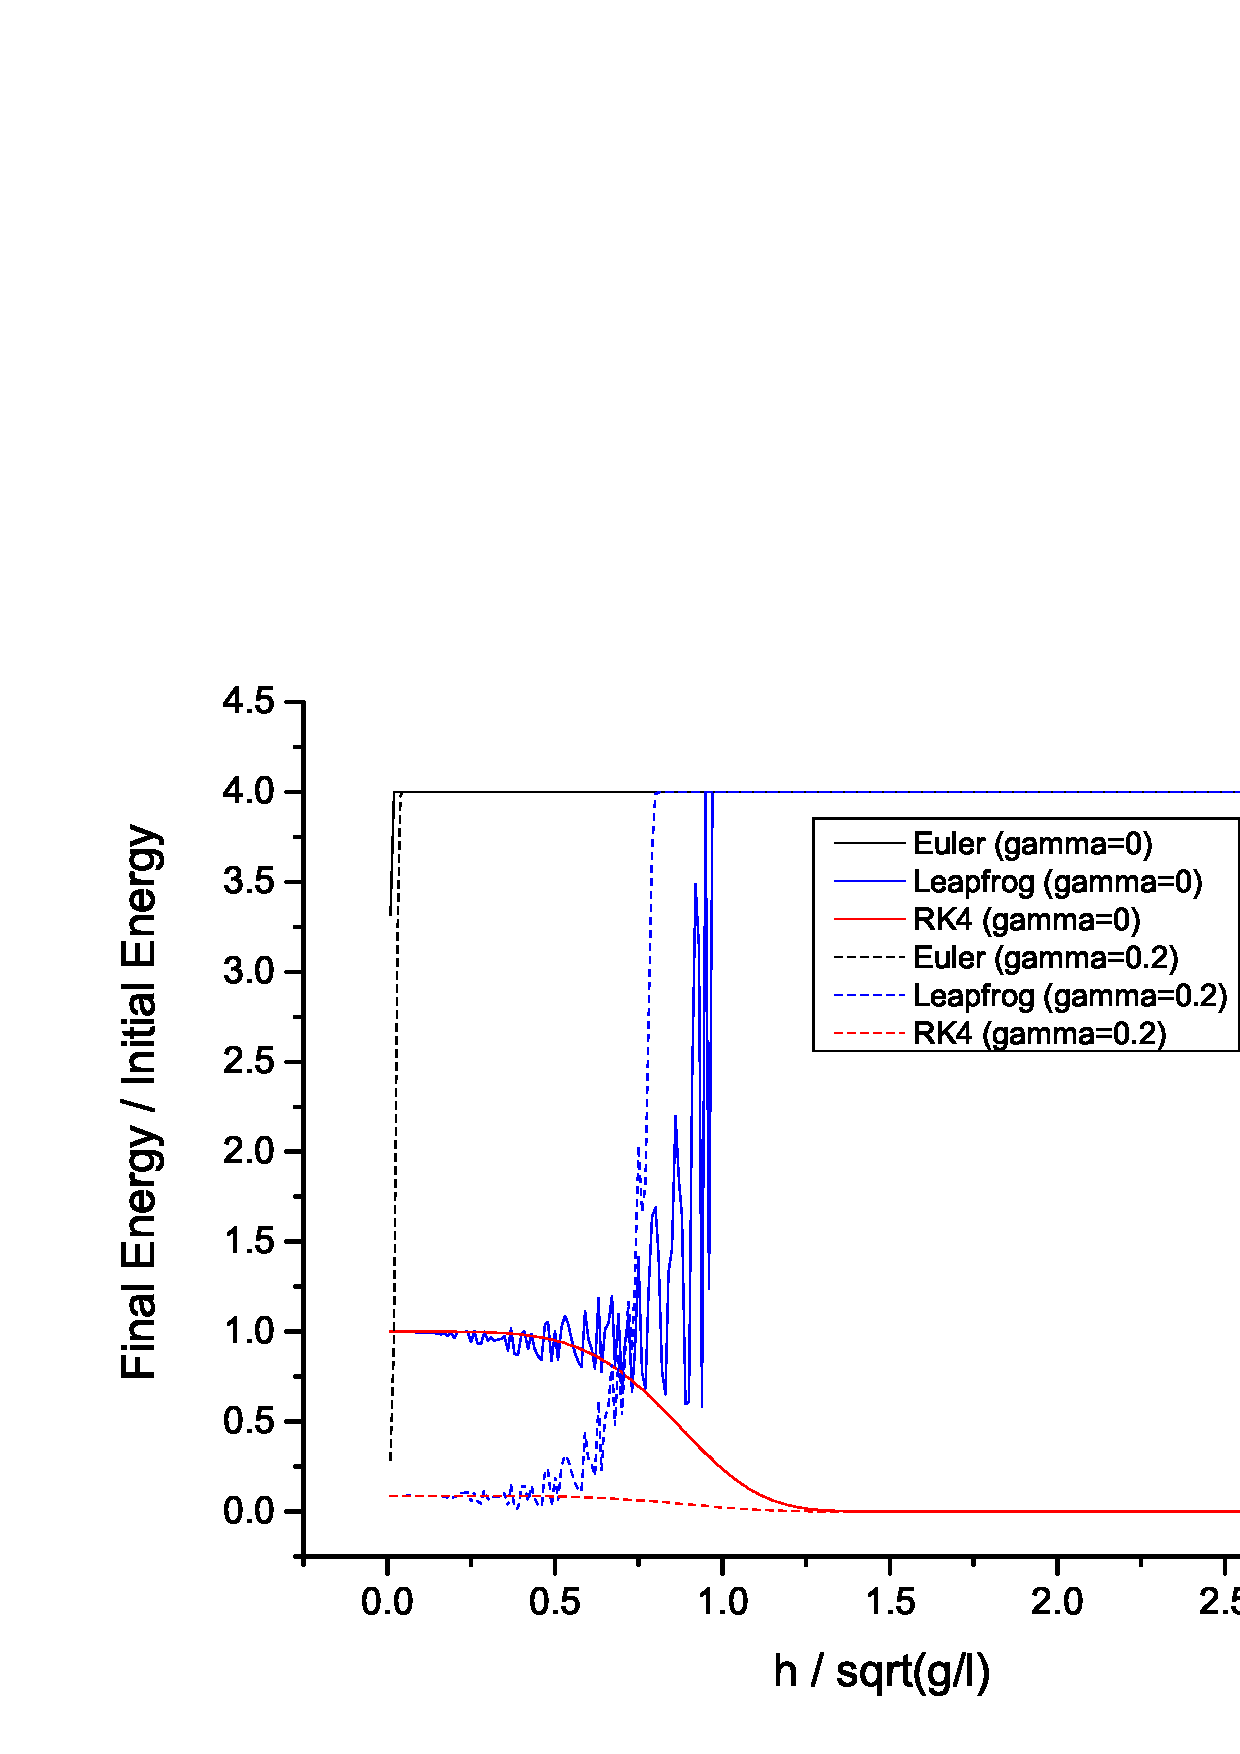
\includegraphics[width=1.1\textwidth]{img/energy_ratio_vs_h.png}
\caption{The ratio of final pendulum energy ($E$ = kinetic + potential) and intial $E$ versus the step size $h$ for the three numerical methods in the undamped case and a lightly damped case ($\gamma$ = 0.2).}
\label{fig:e_vs_h}
\end{figure}

\section{The Double Pendulum}
\subsection{Theory}
\subsubsection*{System Description \& Parameters}
The idealised double pendulum system comprises the single pendulum setup as before with an added bob of mass $M$ attached by a massless rod (also of length $l$) to the first mass which draws an angle from the vertical of $\psi$ as depicted in figure \ref{fig:dp_diag}.

\begin{wrapfigure}{r}{0pt}
\vspace{-20pt}
\hspace{5pt}
\includegraphics[height=0.3\textheight]{img/dp_diag.png}
\caption{The single pendulum notation used throughout this report.}
\label{fig:dp_diag}
\vspace{-30pt}
\end{wrapfigure}

\subsubsection*{Equations of Motion}
\subsubsection*{A Computer Model for the Single Pendulum System}
\subsection{Method}
\subsection{Results \& Discussion}

\end{document}  